\documentclass[10pt,twocolumn,letterpaper]{article}
\usepackage[rebuttal]{cvpr}

% Include other packages here, before hyperref.
\usepackage{graphicx}
\usepackage{amsmath}
\usepackage{amssymb}
\usepackage{booktabs}
\usepackage{graphicx}
\usepackage{caption}
\setlength{\textfloatsep}{6pt}
\setlength{\floatsep}{6pt}
\setlength{\intextsep}{6pt}
\captionsetup{skip=2pt}
\usepackage{multirow}
\usepackage{booktabs}


% Import additional packages in the preamble file, before hyperref
\input{preamble}

% If you comment hyperref and then uncomment it, you should delete
% egpaper.aux before re-running latex.  (Or just hit 'q' on the first latex
% run, let it finish, and you should be clear).
\definecolor{cvprblue}{rgb}{0.21,0.49,0.74}
\usepackage[pagebackref,breaklinks,colorlinks,allcolors=cvprblue]{hyperref}
\renewcommand{\thetable}{R\arabic{table}}
\renewcommand{\thefigure}{R\arabic{figure}}


% Reviewer color definitions (by reviewer ID)
\usepackage{xcolor}

\definecolor{revtK5W}{RGB}{0,70,140}    % tK5W: engineering / experiments
\definecolor{revZ1tg}{RGB}{200,110,0}   % Z1tg: causal / senior
\definecolor{revbqeb}{RGB}{150,0,0}     % bqeb: theory / prior work


% If you wish to avoid re-using figure, table, and equation numbers from
% the main paper, please uncomment the following and change the numbers
% appropriately.
%\setcounter{figure}{2}
%\setcounter{table}{1}
%\setcounter{equation}{2}

% If you wish to avoid re-using reference numbers from the main paper,
% please uncomment the following and change the counter value to the
% number of references you have in the main paper (here, 100).
%\makeatletter
%\apptocmd{\thebibliography}{\global\c@NAT@ctr 100\relax}{}{}
%\makeatother

%%%%%%%%% PAPER ID  - PLEASE UPDATE
\def\paperID{32049} % *** Enter the Paper ID here
\def\confName{CVPR}
\def\confYear{2026}

\begin{document}

%%%%%%%%% TITLE - PLEASE UPDATE
\title{Causality-Aware Direct Preference Optimization for Aligning Medical Vision Language Models}  % **** Enter the paper title here

\maketitle
\thispagestyle{empty}
\appendix

%%%%%%%%% BODY TEXT - ENTER YOUR RESPONSE BELOW
\noindent
%We thank all reviewers for their constructive feedback. We appreciate the recognition of the importance of mitigating background shortcuts in Med-LVLMs (\textcolor{revtK5W}{tK5W}, \textcolor{revZ1tg}{Z1tg}), the causal formulation and theoretical grounding of our preference optimization framework (\textcolor{revZ1tg}{Z1tg}, \textcolor{revbqeb}{bqeb}), and the strong, consistent empirical gains and model-agnostic design demonstrated across benchmarks (\textcolor{revtK5W}{tK5W}, \textcolor{revZ1tg}{Z1tg}, \textcolor{revbqeb}{bqeb}).

We thank all reviewers for their constructive feedback. We appreciate the positive assessment of our work and the insightful suggestions for additional experiments, which help further strengthen and validate the paper. Below we respond to the comments in detail.





\noindent{\textbf{Clarification on key formulas} (\textcolor{revtK5W}{tK5W}, \textcolor{revZ1tg}{Z1tg}).}
We define the causal reward (Eq.~9) as $r_c(x,y):=R_{b,e}(x,y)-R_{b,e^\ast}(x,y)$. Under the KL-regularized maximum-entropy objective, applying the reward--log-policy-ratio identity to the factual ($e$) and the counterfactual environment ($e^\ast$) separately yields
$R_{b,e}(x,y)=\eta^{-1}\log\frac{\pi_e(y\mid x)}{\pi_{\mathrm{ref}}(y\mid x)}+\eta^{-1}\log Z_e(x)$ and $R_{b,e^\ast}(x,y)=\eta^{-1}\log\frac{\pi_{e^\ast}(y\mid x)}{\pi_{\mathrm{ref}}(y\mid x)}+\eta^{-1}\log Z_{e^\ast}(x)$. Subtracting the two expressions gives an explicit form of the causal reward $
r_c(x,y)
=
\eta^{-1}\!\left[
\log \frac{\pi_e(y\mid x)}{\pi_{\mathrm{ref}}(y\mid x)}
-
\log \frac{\pi_{e^\ast}(y\mid x)}{\pi_{\mathrm{ref}}(y\mid x)}
\right]
+
\eta^{-1}\log\frac{Z_e(x)}{Z_{e^\ast}(x)}
$ which cancels the normalization term
since Bradley–Terry likelihoods depend only on pairwise reward differences. 
% Following the standard DPO derivation and replacing the the above equation into Eq. 10, this leads directly to the pairwise log-likelihood difference in Eq.~12 and 13.
Substituting into Eq.~10 and following the standard DPO derivation leads directly
to the pairwise log-likelihood difference in Eq.~12–13.
% This derivation relies on the assumption that the factual and counterfactual policies are latent KL-regularized MaxEnt optima induced by their respective rewards, and that fitting the same optimized policy $\pi_{\theta}$ provides a consistent surrogate of the causal reward contrast.
This derivation assumes that factual and counterfactual policies are latent
KL-regularized MaxEnt optima, and that fitting the same optimized policy $\pi_{\theta}$ provides a
consistent surrogate for the causal reward contrast. Eq. 17 is not meant to be a strictly derived objective, but a heuristic construction for ablation experiments.


\noindent{\textbf{Implementation details} (\textcolor{revZ1tg}{Z1tg})}. Negative response generation and hallucination filtering
follow exactly the same strategy as MMedPO, as stated in Sec. 4.3.1.



\noindent{\textbf{Motivation and causal theory} (\textcolor{revbqeb}{bqeb})}. Our work differs from prior studies that focus on bias mitigation for discriminative VQA models. The underlying counterfactual perspective were introduced in earlier causal theories (e.g., [32, 34]). We extend them to a reinforcement learning / MDP framework for aligning MLLMs, and establish a principled connection between causal reward contrasts and preference-based objectives, supported by both theoretical analysis and optimization. 
% Regarding the causal graph, prior knowledge is implicitly captured by the reference policy $\pi_{\mathrm{ref}}$ and is explicitly reflected in the inference pathways from background $B$ and joint feature $E$ to the reward $R$ (i.e., the $B\rightarrow R$ and $E\rightarrow R$ edges). 
In our causal graph, prior knowledge is implicitly captured by the reference policy
$\pi_{\mathrm{ref}}$ and reflected in the inference pathways from background $B$ and
joint feature $E$ to reward $R$ (i.e., the $B\rightarrow R$ and $E\rightarrow R$ edges).
% As standard in structural causal models, stochastic noise is absorbed into exogenous variables and therefore does not need to be explicitly represented in the graph.
As standard in SCMs, stochastic noise is absorbed into exogenous variables and need not be explicitly represented.


\noindent{\textbf{Composite input validation} (\textcolor{revtK5W}{tK5W}, \textcolor{revZ1tg}{Z1tg})}. 
We clarify that all CaMedPO results reported in the main paper use the standard test-time prompt with the original images. As Shown in Table R1, A1 (also in Table 2) uses composite images with standard prompts at test time, which can be viewed as a weakened or mismatched input condition. When composite images are paired with matched composite prompts (A2), performance remains close to the original CaMedPO results, consistent with the training procedure that explicitly preserves both input forms (Eq.~15). 

\noindent{\textbf{Background shortcut validation (\textcolor{revtK5W}{tK5W}, \textcolor{revZ1tg}{Z1tg})}}. First, we randomly perturb non-lesion regions at test time using models trained with zero-padding (repeated five times); CaMedPO (B1) shows a smaller performance drop and lower variance than MMedPO (B2). Second, training with mixed zero-padding and Gaussian noise in composite images leads to a slight performance gain for CaMedPO. Finally, lesion-removal consistency is evaluated using background-only inputs (Table~2), where CaMedPO exhibits a substantially larger degradation gap, indicating reduced reliance on background cues.


\begin{table}[t]
\centering
\caption{Ablation study results on VQA-RAD and IU-XRay. $t$ denotes model under testing. All models are enhanced with SFT.}
\resizebox{\linewidth}{!}{
\begin{tabular}{c l cc ccc}
\toprule
\multirow{2}{*}{\textbf{ID}} & \multirow{2}{*}{\textbf{Methods}} & 
\multicolumn{2}{c}{\textbf{VQA-RAD}} & 
\multicolumn{3}{c}{\textbf{IU-XRay}} \\
\cmidrule(lr){3-4} \cmidrule(lr){5-7}
 &  & \textbf{Open} & \textbf{Closed} & \textbf{BLEU} & \textbf{ROUGE-L} & \textbf{METEOR} \\
\midrule
-- & LLaVa-Med v1.5 & 29.50 & 64.54 & 14.56 & 10.31 & 10.95 \\
-- & MMedPO & 37.00 & 67.73 & 24.00 & 30.13 & 35.17 \\
-- & CaMedPO & 42.50 & 74.90 & 26.23 & 34.13 & 36.25 \\
\midrule
A1 & CaMedPO$_t$ w/ composite input & 37.50 & 69.32 & 22.35 & 28.69 & 32.57 \\
A2 & CaMedPO$_t$ w/ composite input and prompt & 43.43 & 73.00 & 25.67 & 33.62 & 35.05 \\
\midrule
B1 & MMedPO$_t$ w/ Background swap & $34.00 \pm 2.20$ & $65.14 \pm 1.55$ & 18.45 & 25.21 & 26.02 \\
B2 & CaMedPO$_t$ w/ Background swap & $41.30 \pm 0.58$ & $71.94 \pm 0.76$ & 25.28 & 33.65 & 34.55 \\
\midrule
C1 & CaMedPO$_t$ w/ Gaussian Noise & 43.82 & 73.50 & 26.86 & 34.33 & 36.20 \\
C2 & CaMedPO$_t$ w/ Background swap & $42.70 \pm 0.60$ & $72.82 \pm 0.76$ & 25.67 & 33.85 & 35.62 \\
\bottomrule
\end{tabular}
}
\end{table}




\iffalse
\begin{table}[t]
\centering
\caption{RadGraph F1 scores on IU-Xray dataset.}
\label{tab:radgraph_f1}
\resizebox{0.5\linewidth}{!}{
\begin{tabular}{lccc}
\toprule
\textbf{Model} & \textbf{Simple-F1} & \textbf{Partial-F1} & \textbf{Complete-F1} \\
\midrule
LLaVA-Med & 11.27 & 10.99 & 10.40 \\
LLaVA-Med$^{\mathrm{s}}$ & 30.32 & 26.22 & 16.77 \\
LLaVA-Med$^{\mathrm{s}}$ w/ DPO & 31.11 & 27.06 & 19.12 \\
MMedPO$^{\mathrm{s}}$ & 26.33 & 22.55 & 15.68 \\
CaMedPO$^{\mathrm{s}}$ & 35.23 & 32.18 & 21.42 \\
\bottomrule
\end{tabular}
}
\end{table}


\begin{figure}[t]
    \centering
    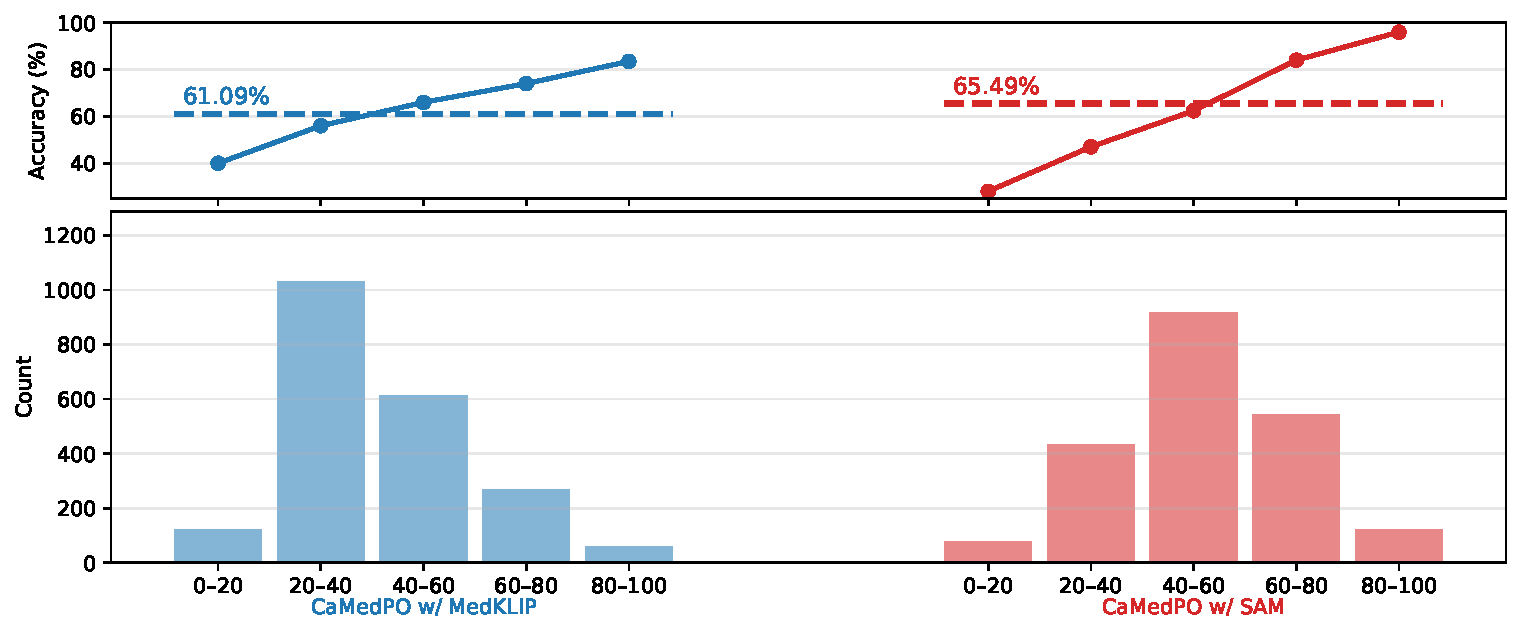
\includegraphics[width=0.4\textwidth]{figs/segmentation.pdf}
    \caption{
    % Examples demonstrating the reasonable responses generated by CaMedPO.
    Segmentation performance analysis on SLAKE.
    }
    \label{fig:seg}
    \vspace{-10pt}
\end{figure}
\fi

\begin{figure}[t]
\centering
\begin{minipage}{0.45\linewidth} 
    \centering
    \captionof{table}{RadGraph F1 scores on IU-Xray dataset.}
    \label{tab:radgraph_f1}
    \resizebox{\linewidth}{!}{
    \begin{tabular}{lccc}
    \toprule
    \textbf{Model} & \textbf{Simple-F1} & \textbf{Partial-F1} & \textbf{Complete-F1} \\
    \midrule
    LLaVA-Med & 11.27 & 10.99 & 10.40 \\
    LLaVA-Med$^{\mathrm{s}}$ & 30.32 & 26.22 & 16.77 \\
    LLaVA-Med$^{\mathrm{s}}$ w/ DPO & 31.11 & 27.06 & 19.12 \\
    MMedPO$^{\mathrm{s}}$ & 26.33 & 22.55 & 15.68 \\
    CaMedPO$^{\mathrm{s}}$ & 35.23 & 32.18 & 21.42 \\
    \bottomrule
    \end{tabular}
    }
\end{minipage}
\hspace{0.02\linewidth} 
\begin{minipage}{0.45\linewidth} 
    \centering
    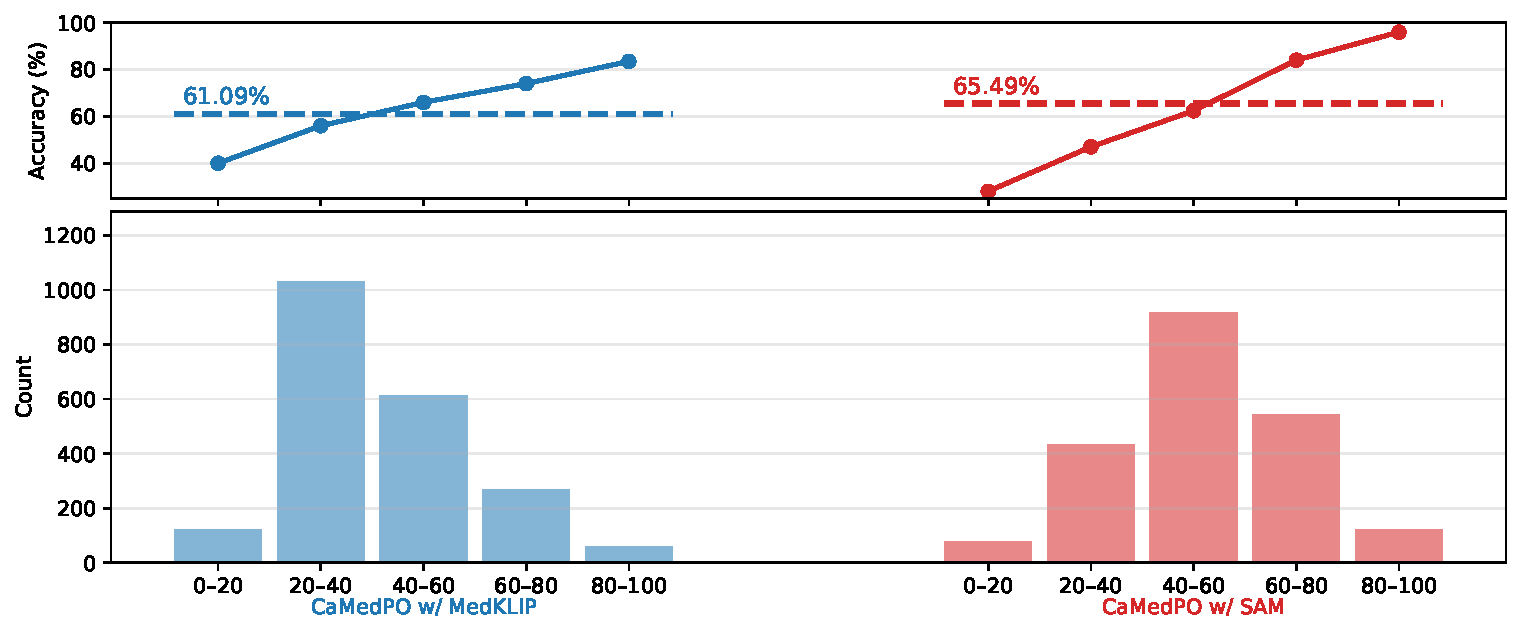
\includegraphics[width=1.1\linewidth]{figs/segmentation.pdf}
    \captionof{figure}{Segmentation performance analysis.}
    \label{fig:seg}
\end{minipage}
\end{figure}



\noindent{\textbf{Medical-fact evidence for report generation} (\textcolor{revZ1tg}{Z1tg})}. We report structured RadGraph F1 scores on the IU-Xray test set (Table~R2). CaMedPO consistently outperforms all baselines, demonstrating improved factual correctness.

\noindent{\textbf{Segmentation analysis} (\textcolor{revtK5W}{tK5W}). 
% We analyze the impact of segmentation quality on test-time performance via IoU evaluation against annotated lesions on SLAKE(Fig. R1), with accuracy computed over both open- and closed-ended questions. We use composite inputs at test time to evaluate the impact. 
We evaluate the impact of segmentation quality on test-time performance via IoU
against annotated lesions on SLAKE (Fig.~R1), reporting accuracy on both open-
and closed-ended questions using composite inputs at test time.
% The results show that inaccurate lesion segmentation can interfere with preference signals and degrade performance, especially for stronger models. Meanwhile, better segmentation tool can help improving the overall performance (Table 2 and Fig. R1). 
We find that inaccurate lesion segmentation interferes with preference signals and degrades performance,
especially for stronger models, while better segmentation tool consistently improves overall performance (Table~2, Fig.~R1).

\noindent\textbf{Generalization and distribution shift} (\textcolor{revtK5W}{tK5W}). 
We clarify that our claim is mitigating background shortcut and therefore evaluate under background interventions that simulate distribution shifts (Table~R1). Evaluating cross-hospital shifts is left to future work due to limited rebuttal period.

\noindent{\textbf{Compatibility analysis on other LVLMs} (\textcolor{revbqeb}{bqeb}). 
% We conducted experiments in S5.2 to evaluate CaMedPO is transferable to different base models. 
We evaluate transferability across different base models in Sec. S5.2 (Fig. 6), with more in-depth analysis in supplementary material and rebuttal.
% Moreover, we have conducted more in-depth analysis in suppl. and rebuttal.











\end{document}